\documentclass[11pt]{article}

    \usepackage[breakable]{tcolorbox}
    \usepackage{parskip} % Stop auto-indenting (to mimic markdown behaviour)
    

    % Basic figure setup, for now with no caption control since it's done
    % automatically by Pandoc (which extracts ![](path) syntax from Markdown).
    \usepackage{graphicx}
    % Keep aspect ratio if custom image width or height is specified
    \setkeys{Gin}{keepaspectratio}
    % Maintain compatibility with old templates. Remove in nbconvert 6.0
    \let\Oldincludegraphics\includegraphics
    % Ensure that by default, figures have no caption (until we provide a
    % proper Figure object with a Caption API and a way to capture that
    % in the conversion process - todo).
    \usepackage{caption}
    \DeclareCaptionFormat{nocaption}{}
    \captionsetup{format=nocaption,aboveskip=0pt,belowskip=0pt}

    \usepackage{float}
    \floatplacement{figure}{H} % forces figures to be placed at the correct location
    \usepackage{xcolor} % Allow colors to be defined
    \usepackage{enumerate} % Needed for markdown enumerations to work
    \usepackage{geometry} % Used to adjust the document margins
    \usepackage{amsmath} % Equations
    \usepackage{amssymb} % Equations
    \usepackage{textcomp} % defines textquotesingle
    % Hack from http://tex.stackexchange.com/a/47451/13684:
    \AtBeginDocument{%
        \def\PYZsq{\textquotesingle}% Upright quotes in Pygmentized code
    }
    \usepackage{upquote} % Upright quotes for verbatim code
    \usepackage{eurosym} % defines \euro

    \usepackage{iftex}
    \ifPDFTeX
        \usepackage[T1]{fontenc}
        \IfFileExists{alphabeta.sty}{
              \usepackage{alphabeta}
          }{
              \usepackage[mathletters]{ucs}
              \usepackage[utf8x]{inputenc}
          }
    \else
        \usepackage{fontspec}
        \usepackage{unicode-math}
    \fi

    \usepackage{fancyvrb} % verbatim replacement that allows latex
    \usepackage{grffile} % extends the file name processing of package graphics
                         % to support a larger range
    \makeatletter % fix for old versions of grffile with XeLaTeX
    \@ifpackagelater{grffile}{2019/11/01}
    {
      % Do nothing on new versions
    }
    {
      \def\Gread@@xetex#1{%
        \IfFileExists{"\Gin@base".bb}%
        {\Gread@eps{\Gin@base.bb}}%
        {\Gread@@xetex@aux#1}%
      }
    }
    \makeatother
    \usepackage[Export]{adjustbox} % Used to constrain images to a maximum size
    \adjustboxset{max size={0.9\linewidth}{0.9\paperheight}}

    % The hyperref package gives us a pdf with properly built
    % internal navigation ('pdf bookmarks' for the table of contents,
    % internal cross-reference links, web links for URLs, etc.)
    \usepackage{hyperref}
    % The default LaTeX title has an obnoxious amount of whitespace. By default,
    % titling removes some of it. It also provides customization options.
    \usepackage{titling}
    \usepackage{longtable} % longtable support required by pandoc >1.10
    \usepackage{booktabs}  % table support for pandoc > 1.12.2
    \usepackage{array}     % table support for pandoc >= 2.11.3
    \usepackage{calc}      % table minipage width calculation for pandoc >= 2.11.1
    \usepackage[inline]{enumitem} % IRkernel/repr support (it uses the enumerate* environment)
    \usepackage[normalem]{ulem} % ulem is needed to support strikethroughs (\sout)
                                % normalem makes italics be italics, not underlines
    \usepackage{soul}      % strikethrough (\st) support for pandoc >= 3.0.0
    \usepackage{mathrsfs}
    

    
    % Colors for the hyperref package
    \definecolor{urlcolor}{rgb}{0,.145,.698}
    \definecolor{linkcolor}{rgb}{.71,0.21,0.01}
    \definecolor{citecolor}{rgb}{.12,.54,.11}

    % ANSI colors
    \definecolor{ansi-black}{HTML}{3E424D}
    \definecolor{ansi-black-intense}{HTML}{282C36}
    \definecolor{ansi-red}{HTML}{E75C58}
    \definecolor{ansi-red-intense}{HTML}{B22B31}
    \definecolor{ansi-green}{HTML}{00A250}
    \definecolor{ansi-green-intense}{HTML}{007427}
    \definecolor{ansi-yellow}{HTML}{DDB62B}
    \definecolor{ansi-yellow-intense}{HTML}{B27D12}
    \definecolor{ansi-blue}{HTML}{208FFB}
    \definecolor{ansi-blue-intense}{HTML}{0065CA}
    \definecolor{ansi-magenta}{HTML}{D160C4}
    \definecolor{ansi-magenta-intense}{HTML}{A03196}
    \definecolor{ansi-cyan}{HTML}{60C6C8}
    \definecolor{ansi-cyan-intense}{HTML}{258F8F}
    \definecolor{ansi-white}{HTML}{C5C1B4}
    \definecolor{ansi-white-intense}{HTML}{A1A6B2}
    \definecolor{ansi-default-inverse-fg}{HTML}{FFFFFF}
    \definecolor{ansi-default-inverse-bg}{HTML}{000000}

    % common color for the border for error outputs.
    \definecolor{outerrorbackground}{HTML}{FFDFDF}

    % commands and environments needed by pandoc snippets
    % extracted from the output of `pandoc -s`
    \providecommand{\tightlist}{%
      \setlength{\itemsep}{0pt}\setlength{\parskip}{0pt}}
    \DefineVerbatimEnvironment{Highlighting}{Verbatim}{commandchars=\\\{\}}
    % Add ',fontsize=\small' for more characters per line
    \newenvironment{Shaded}{}{}
    \newcommand{\KeywordTok}[1]{\textcolor[rgb]{0.00,0.44,0.13}{\textbf{{#1}}}}
    \newcommand{\DataTypeTok}[1]{\textcolor[rgb]{0.56,0.13,0.00}{{#1}}}
    \newcommand{\DecValTok}[1]{\textcolor[rgb]{0.25,0.63,0.44}{{#1}}}
    \newcommand{\BaseNTok}[1]{\textcolor[rgb]{0.25,0.63,0.44}{{#1}}}
    \newcommand{\FloatTok}[1]{\textcolor[rgb]{0.25,0.63,0.44}{{#1}}}
    \newcommand{\CharTok}[1]{\textcolor[rgb]{0.25,0.44,0.63}{{#1}}}
    \newcommand{\StringTok}[1]{\textcolor[rgb]{0.25,0.44,0.63}{{#1}}}
    \newcommand{\CommentTok}[1]{\textcolor[rgb]{0.38,0.63,0.69}{\textit{{#1}}}}
    \newcommand{\OtherTok}[1]{\textcolor[rgb]{0.00,0.44,0.13}{{#1}}}
    \newcommand{\AlertTok}[1]{\textcolor[rgb]{1.00,0.00,0.00}{\textbf{{#1}}}}
    \newcommand{\FunctionTok}[1]{\textcolor[rgb]{0.02,0.16,0.49}{{#1}}}
    \newcommand{\RegionMarkerTok}[1]{{#1}}
    \newcommand{\ErrorTok}[1]{\textcolor[rgb]{1.00,0.00,0.00}{\textbf{{#1}}}}
    \newcommand{\NormalTok}[1]{{#1}}

    % Additional commands for more recent versions of Pandoc
    \newcommand{\ConstantTok}[1]{\textcolor[rgb]{0.53,0.00,0.00}{{#1}}}
    \newcommand{\SpecialCharTok}[1]{\textcolor[rgb]{0.25,0.44,0.63}{{#1}}}
    \newcommand{\VerbatimStringTok}[1]{\textcolor[rgb]{0.25,0.44,0.63}{{#1}}}
    \newcommand{\SpecialStringTok}[1]{\textcolor[rgb]{0.73,0.40,0.53}{{#1}}}
    \newcommand{\ImportTok}[1]{{#1}}
    \newcommand{\DocumentationTok}[1]{\textcolor[rgb]{0.73,0.13,0.13}{\textit{{#1}}}}
    \newcommand{\AnnotationTok}[1]{\textcolor[rgb]{0.38,0.63,0.69}{\textbf{\textit{{#1}}}}}
    \newcommand{\CommentVarTok}[1]{\textcolor[rgb]{0.38,0.63,0.69}{\textbf{\textit{{#1}}}}}
    \newcommand{\VariableTok}[1]{\textcolor[rgb]{0.10,0.09,0.49}{{#1}}}
    \newcommand{\ControlFlowTok}[1]{\textcolor[rgb]{0.00,0.44,0.13}{\textbf{{#1}}}}
    \newcommand{\OperatorTok}[1]{\textcolor[rgb]{0.40,0.40,0.40}{{#1}}}
    \newcommand{\BuiltInTok}[1]{{#1}}
    \newcommand{\ExtensionTok}[1]{{#1}}
    \newcommand{\PreprocessorTok}[1]{\textcolor[rgb]{0.74,0.48,0.00}{{#1}}}
    \newcommand{\AttributeTok}[1]{\textcolor[rgb]{0.49,0.56,0.16}{{#1}}}
    \newcommand{\InformationTok}[1]{\textcolor[rgb]{0.38,0.63,0.69}{\textbf{\textit{{#1}}}}}
    \newcommand{\WarningTok}[1]{\textcolor[rgb]{0.38,0.63,0.69}{\textbf{\textit{{#1}}}}}


    % Define a nice break command that doesn't care if a line doesn't already
    % exist.
    \def\br{\hspace*{\fill} \\* }
    % Math Jax compatibility definitions
    \def\gt{>}
    \def\lt{<}
    \let\Oldtex\TeX
    \let\Oldlatex\LaTeX
    \renewcommand{\TeX}{\textrm{\Oldtex}}
    \renewcommand{\LaTeX}{\textrm{\Oldlatex}}
    % Document parameters
    % Document title
    \title{plotting}
    
    
    
    
    
    
    
% Pygments definitions
\makeatletter
\def\PY@reset{\let\PY@it=\relax \let\PY@bf=\relax%
    \let\PY@ul=\relax \let\PY@tc=\relax%
    \let\PY@bc=\relax \let\PY@ff=\relax}
\def\PY@tok#1{\csname PY@tok@#1\endcsname}
\def\PY@toks#1+{\ifx\relax#1\empty\else%
    \PY@tok{#1}\expandafter\PY@toks\fi}
\def\PY@do#1{\PY@bc{\PY@tc{\PY@ul{%
    \PY@it{\PY@bf{\PY@ff{#1}}}}}}}
\def\PY#1#2{\PY@reset\PY@toks#1+\relax+\PY@do{#2}}

\@namedef{PY@tok@w}{\def\PY@tc##1{\textcolor[rgb]{0.73,0.73,0.73}{##1}}}
\@namedef{PY@tok@c}{\let\PY@it=\textit\def\PY@tc##1{\textcolor[rgb]{0.24,0.48,0.48}{##1}}}
\@namedef{PY@tok@cp}{\def\PY@tc##1{\textcolor[rgb]{0.61,0.40,0.00}{##1}}}
\@namedef{PY@tok@k}{\let\PY@bf=\textbf\def\PY@tc##1{\textcolor[rgb]{0.00,0.50,0.00}{##1}}}
\@namedef{PY@tok@kp}{\def\PY@tc##1{\textcolor[rgb]{0.00,0.50,0.00}{##1}}}
\@namedef{PY@tok@kt}{\def\PY@tc##1{\textcolor[rgb]{0.69,0.00,0.25}{##1}}}
\@namedef{PY@tok@o}{\def\PY@tc##1{\textcolor[rgb]{0.40,0.40,0.40}{##1}}}
\@namedef{PY@tok@ow}{\let\PY@bf=\textbf\def\PY@tc##1{\textcolor[rgb]{0.67,0.13,1.00}{##1}}}
\@namedef{PY@tok@nb}{\def\PY@tc##1{\textcolor[rgb]{0.00,0.50,0.00}{##1}}}
\@namedef{PY@tok@nf}{\def\PY@tc##1{\textcolor[rgb]{0.00,0.00,1.00}{##1}}}
\@namedef{PY@tok@nc}{\let\PY@bf=\textbf\def\PY@tc##1{\textcolor[rgb]{0.00,0.00,1.00}{##1}}}
\@namedef{PY@tok@nn}{\let\PY@bf=\textbf\def\PY@tc##1{\textcolor[rgb]{0.00,0.00,1.00}{##1}}}
\@namedef{PY@tok@ne}{\let\PY@bf=\textbf\def\PY@tc##1{\textcolor[rgb]{0.80,0.25,0.22}{##1}}}
\@namedef{PY@tok@nv}{\def\PY@tc##1{\textcolor[rgb]{0.10,0.09,0.49}{##1}}}
\@namedef{PY@tok@no}{\def\PY@tc##1{\textcolor[rgb]{0.53,0.00,0.00}{##1}}}
\@namedef{PY@tok@nl}{\def\PY@tc##1{\textcolor[rgb]{0.46,0.46,0.00}{##1}}}
\@namedef{PY@tok@ni}{\let\PY@bf=\textbf\def\PY@tc##1{\textcolor[rgb]{0.44,0.44,0.44}{##1}}}
\@namedef{PY@tok@na}{\def\PY@tc##1{\textcolor[rgb]{0.41,0.47,0.13}{##1}}}
\@namedef{PY@tok@nt}{\let\PY@bf=\textbf\def\PY@tc##1{\textcolor[rgb]{0.00,0.50,0.00}{##1}}}
\@namedef{PY@tok@nd}{\def\PY@tc##1{\textcolor[rgb]{0.67,0.13,1.00}{##1}}}
\@namedef{PY@tok@s}{\def\PY@tc##1{\textcolor[rgb]{0.73,0.13,0.13}{##1}}}
\@namedef{PY@tok@sd}{\let\PY@it=\textit\def\PY@tc##1{\textcolor[rgb]{0.73,0.13,0.13}{##1}}}
\@namedef{PY@tok@si}{\let\PY@bf=\textbf\def\PY@tc##1{\textcolor[rgb]{0.64,0.35,0.47}{##1}}}
\@namedef{PY@tok@se}{\let\PY@bf=\textbf\def\PY@tc##1{\textcolor[rgb]{0.67,0.36,0.12}{##1}}}
\@namedef{PY@tok@sr}{\def\PY@tc##1{\textcolor[rgb]{0.64,0.35,0.47}{##1}}}
\@namedef{PY@tok@ss}{\def\PY@tc##1{\textcolor[rgb]{0.10,0.09,0.49}{##1}}}
\@namedef{PY@tok@sx}{\def\PY@tc##1{\textcolor[rgb]{0.00,0.50,0.00}{##1}}}
\@namedef{PY@tok@m}{\def\PY@tc##1{\textcolor[rgb]{0.40,0.40,0.40}{##1}}}
\@namedef{PY@tok@gh}{\let\PY@bf=\textbf\def\PY@tc##1{\textcolor[rgb]{0.00,0.00,0.50}{##1}}}
\@namedef{PY@tok@gu}{\let\PY@bf=\textbf\def\PY@tc##1{\textcolor[rgb]{0.50,0.00,0.50}{##1}}}
\@namedef{PY@tok@gd}{\def\PY@tc##1{\textcolor[rgb]{0.63,0.00,0.00}{##1}}}
\@namedef{PY@tok@gi}{\def\PY@tc##1{\textcolor[rgb]{0.00,0.52,0.00}{##1}}}
\@namedef{PY@tok@gr}{\def\PY@tc##1{\textcolor[rgb]{0.89,0.00,0.00}{##1}}}
\@namedef{PY@tok@ge}{\let\PY@it=\textit}
\@namedef{PY@tok@gs}{\let\PY@bf=\textbf}
\@namedef{PY@tok@ges}{\let\PY@bf=\textbf\let\PY@it=\textit}
\@namedef{PY@tok@gp}{\let\PY@bf=\textbf\def\PY@tc##1{\textcolor[rgb]{0.00,0.00,0.50}{##1}}}
\@namedef{PY@tok@go}{\def\PY@tc##1{\textcolor[rgb]{0.44,0.44,0.44}{##1}}}
\@namedef{PY@tok@gt}{\def\PY@tc##1{\textcolor[rgb]{0.00,0.27,0.87}{##1}}}
\@namedef{PY@tok@err}{\def\PY@bc##1{{\setlength{\fboxsep}{\string -\fboxrule}\fcolorbox[rgb]{1.00,0.00,0.00}{1,1,1}{\strut ##1}}}}
\@namedef{PY@tok@kc}{\let\PY@bf=\textbf\def\PY@tc##1{\textcolor[rgb]{0.00,0.50,0.00}{##1}}}
\@namedef{PY@tok@kd}{\let\PY@bf=\textbf\def\PY@tc##1{\textcolor[rgb]{0.00,0.50,0.00}{##1}}}
\@namedef{PY@tok@kn}{\let\PY@bf=\textbf\def\PY@tc##1{\textcolor[rgb]{0.00,0.50,0.00}{##1}}}
\@namedef{PY@tok@kr}{\let\PY@bf=\textbf\def\PY@tc##1{\textcolor[rgb]{0.00,0.50,0.00}{##1}}}
\@namedef{PY@tok@bp}{\def\PY@tc##1{\textcolor[rgb]{0.00,0.50,0.00}{##1}}}
\@namedef{PY@tok@fm}{\def\PY@tc##1{\textcolor[rgb]{0.00,0.00,1.00}{##1}}}
\@namedef{PY@tok@vc}{\def\PY@tc##1{\textcolor[rgb]{0.10,0.09,0.49}{##1}}}
\@namedef{PY@tok@vg}{\def\PY@tc##1{\textcolor[rgb]{0.10,0.09,0.49}{##1}}}
\@namedef{PY@tok@vi}{\def\PY@tc##1{\textcolor[rgb]{0.10,0.09,0.49}{##1}}}
\@namedef{PY@tok@vm}{\def\PY@tc##1{\textcolor[rgb]{0.10,0.09,0.49}{##1}}}
\@namedef{PY@tok@sa}{\def\PY@tc##1{\textcolor[rgb]{0.73,0.13,0.13}{##1}}}
\@namedef{PY@tok@sb}{\def\PY@tc##1{\textcolor[rgb]{0.73,0.13,0.13}{##1}}}
\@namedef{PY@tok@sc}{\def\PY@tc##1{\textcolor[rgb]{0.73,0.13,0.13}{##1}}}
\@namedef{PY@tok@dl}{\def\PY@tc##1{\textcolor[rgb]{0.73,0.13,0.13}{##1}}}
\@namedef{PY@tok@s2}{\def\PY@tc##1{\textcolor[rgb]{0.73,0.13,0.13}{##1}}}
\@namedef{PY@tok@sh}{\def\PY@tc##1{\textcolor[rgb]{0.73,0.13,0.13}{##1}}}
\@namedef{PY@tok@s1}{\def\PY@tc##1{\textcolor[rgb]{0.73,0.13,0.13}{##1}}}
\@namedef{PY@tok@mb}{\def\PY@tc##1{\textcolor[rgb]{0.40,0.40,0.40}{##1}}}
\@namedef{PY@tok@mf}{\def\PY@tc##1{\textcolor[rgb]{0.40,0.40,0.40}{##1}}}
\@namedef{PY@tok@mh}{\def\PY@tc##1{\textcolor[rgb]{0.40,0.40,0.40}{##1}}}
\@namedef{PY@tok@mi}{\def\PY@tc##1{\textcolor[rgb]{0.40,0.40,0.40}{##1}}}
\@namedef{PY@tok@il}{\def\PY@tc##1{\textcolor[rgb]{0.40,0.40,0.40}{##1}}}
\@namedef{PY@tok@mo}{\def\PY@tc##1{\textcolor[rgb]{0.40,0.40,0.40}{##1}}}
\@namedef{PY@tok@ch}{\let\PY@it=\textit\def\PY@tc##1{\textcolor[rgb]{0.24,0.48,0.48}{##1}}}
\@namedef{PY@tok@cm}{\let\PY@it=\textit\def\PY@tc##1{\textcolor[rgb]{0.24,0.48,0.48}{##1}}}
\@namedef{PY@tok@cpf}{\let\PY@it=\textit\def\PY@tc##1{\textcolor[rgb]{0.24,0.48,0.48}{##1}}}
\@namedef{PY@tok@c1}{\let\PY@it=\textit\def\PY@tc##1{\textcolor[rgb]{0.24,0.48,0.48}{##1}}}
\@namedef{PY@tok@cs}{\let\PY@it=\textit\def\PY@tc##1{\textcolor[rgb]{0.24,0.48,0.48}{##1}}}

\def\PYZbs{\char`\\}
\def\PYZus{\char`\_}
\def\PYZob{\char`\{}
\def\PYZcb{\char`\}}
\def\PYZca{\char`\^}
\def\PYZam{\char`\&}
\def\PYZlt{\char`\<}
\def\PYZgt{\char`\>}
\def\PYZsh{\char`\#}
\def\PYZpc{\char`\%}
\def\PYZdl{\char`\$}
\def\PYZhy{\char`\-}
\def\PYZsq{\char`\'}
\def\PYZdq{\char`\"}
\def\PYZti{\char`\~}
% for compatibility with earlier versions
\def\PYZat{@}
\def\PYZlb{[}
\def\PYZrb{]}
\makeatother


    % For linebreaks inside Verbatim environment from package fancyvrb.
    \makeatletter
        \newbox\Wrappedcontinuationbox
        \newbox\Wrappedvisiblespacebox
        \newcommand*\Wrappedvisiblespace {\textcolor{red}{\textvisiblespace}}
        \newcommand*\Wrappedcontinuationsymbol {\textcolor{red}{\llap{\tiny$\m@th\hookrightarrow$}}}
        \newcommand*\Wrappedcontinuationindent {3ex }
        \newcommand*\Wrappedafterbreak {\kern\Wrappedcontinuationindent\copy\Wrappedcontinuationbox}
        % Take advantage of the already applied Pygments mark-up to insert
        % potential linebreaks for TeX processing.
        %        {, <, #, %, $, ' and ": go to next line.
        %        _, }, ^, &, >, - and ~: stay at end of broken line.
        % Use of \textquotesingle for straight quote.
        \newcommand*\Wrappedbreaksatspecials {%
            \def\PYGZus{\discretionary{\char`\_}{\Wrappedafterbreak}{\char`\_}}%
            \def\PYGZob{\discretionary{}{\Wrappedafterbreak\char`\{}{\char`\{}}%
            \def\PYGZcb{\discretionary{\char`\}}{\Wrappedafterbreak}{\char`\}}}%
            \def\PYGZca{\discretionary{\char`\^}{\Wrappedafterbreak}{\char`\^}}%
            \def\PYGZam{\discretionary{\char`\&}{\Wrappedafterbreak}{\char`\&}}%
            \def\PYGZlt{\discretionary{}{\Wrappedafterbreak\char`\<}{\char`\<}}%
            \def\PYGZgt{\discretionary{\char`\>}{\Wrappedafterbreak}{\char`\>}}%
            \def\PYGZsh{\discretionary{}{\Wrappedafterbreak\char`\#}{\char`\#}}%
            \def\PYGZpc{\discretionary{}{\Wrappedafterbreak\char`\%}{\char`\%}}%
            \def\PYGZdl{\discretionary{}{\Wrappedafterbreak\char`\$}{\char`\$}}%
            \def\PYGZhy{\discretionary{\char`\-}{\Wrappedafterbreak}{\char`\-}}%
            \def\PYGZsq{\discretionary{}{\Wrappedafterbreak\textquotesingle}{\textquotesingle}}%
            \def\PYGZdq{\discretionary{}{\Wrappedafterbreak\char`\"}{\char`\"}}%
            \def\PYGZti{\discretionary{\char`\~}{\Wrappedafterbreak}{\char`\~}}%
        }
        % Some characters . , ; ? ! / are not pygmentized.
        % This macro makes them "active" and they will insert potential linebreaks
        \newcommand*\Wrappedbreaksatpunct {%
            \lccode`\~`\.\lowercase{\def~}{\discretionary{\hbox{\char`\.}}{\Wrappedafterbreak}{\hbox{\char`\.}}}%
            \lccode`\~`\,\lowercase{\def~}{\discretionary{\hbox{\char`\,}}{\Wrappedafterbreak}{\hbox{\char`\,}}}%
            \lccode`\~`\;\lowercase{\def~}{\discretionary{\hbox{\char`\;}}{\Wrappedafterbreak}{\hbox{\char`\;}}}%
            \lccode`\~`\:\lowercase{\def~}{\discretionary{\hbox{\char`\:}}{\Wrappedafterbreak}{\hbox{\char`\:}}}%
            \lccode`\~`\?\lowercase{\def~}{\discretionary{\hbox{\char`\?}}{\Wrappedafterbreak}{\hbox{\char`\?}}}%
            \lccode`\~`\!\lowercase{\def~}{\discretionary{\hbox{\char`\!}}{\Wrappedafterbreak}{\hbox{\char`\!}}}%
            \lccode`\~`\/\lowercase{\def~}{\discretionary{\hbox{\char`\/}}{\Wrappedafterbreak}{\hbox{\char`\/}}}%
            \catcode`\.\active
            \catcode`\,\active
            \catcode`\;\active
            \catcode`\:\active
            \catcode`\?\active
            \catcode`\!\active
            \catcode`\/\active
            \lccode`\~`\~
        }
    \makeatother

    \let\OriginalVerbatim=\Verbatim
    \makeatletter
    \renewcommand{\Verbatim}[1][1]{%
        %\parskip\z@skip
        \sbox\Wrappedcontinuationbox {\Wrappedcontinuationsymbol}%
        \sbox\Wrappedvisiblespacebox {\FV@SetupFont\Wrappedvisiblespace}%
        \def\FancyVerbFormatLine ##1{\hsize\linewidth
            \vtop{\raggedright\hyphenpenalty\z@\exhyphenpenalty\z@
                \doublehyphendemerits\z@\finalhyphendemerits\z@
                \strut ##1\strut}%
        }%
        % If the linebreak is at a space, the latter will be displayed as visible
        % space at end of first line, and a continuation symbol starts next line.
        % Stretch/shrink are however usually zero for typewriter font.
        \def\FV@Space {%
            \nobreak\hskip\z@ plus\fontdimen3\font minus\fontdimen4\font
            \discretionary{\copy\Wrappedvisiblespacebox}{\Wrappedafterbreak}
            {\kern\fontdimen2\font}%
        }%

        % Allow breaks at special characters using \PYG... macros.
        \Wrappedbreaksatspecials
        % Breaks at punctuation characters . , ; ? ! and / need catcode=\active
        \OriginalVerbatim[#1,codes*=\Wrappedbreaksatpunct]%
    }
    \makeatother

    % Exact colors from NB
    \definecolor{incolor}{HTML}{303F9F}
    \definecolor{outcolor}{HTML}{D84315}
    \definecolor{cellborder}{HTML}{CFCFCF}
    \definecolor{cellbackground}{HTML}{F7F7F7}

    % prompt
    \makeatletter
    \newcommand{\boxspacing}{\kern\kvtcb@left@rule\kern\kvtcb@boxsep}
    \makeatother
    \newcommand{\prompt}[4]{
        {\ttfamily\llap{{\color{#2}[#3]:\hspace{3pt}#4}}\vspace{-\baselineskip}}
    }
    

    
    % Prevent overflowing lines due to hard-to-break entities
    \sloppy
    % Setup hyperref package
    \hypersetup{
      breaklinks=true,  % so long urls are correctly broken across lines
      colorlinks=true,
      urlcolor=urlcolor,
      linkcolor=linkcolor,
      citecolor=citecolor,
      }
    % Slightly bigger margins than the latex defaults
    
    \geometry{verbose,tmargin=1in,bmargin=1in,lmargin=1in,rmargin=1in}
    
    

\begin{document}
    
    \maketitle
    
    

    
    \section{1. An Introduction To Data Visualization In
Python}\label{an-introduction-to-data-visualization-in-python}

This book will cover the most relevant and unique attributes and
features for 9 different Python libraries, before going on to
demonstrate how to visualize data with them. This book will also cover
the different types of data you can visualize in Python, in addition to
common visualization techniques, tools, and plot types.

Before delving too deeply into the libraries themselves, it would be
helpful to gain an intuition of how the landscape of Python's
visualization libraries breaks down. To put that another way, it's
helpful to understand how the different Python libraries are designed
and related to one another. Understanding how the different libraries
operate will help you choose the best library for your visualization
project.

There are a number of different data visualization libraries and modules
compatible with Python. Most of the Python data visualization libraries
can be placed into one of four groups, separated based on their origins
and focus.

The groups are:

• Matplotlib-based libraries\\
• JavaScript libraries\\
• JSON libraries\\
• WebGL libraries

\subsection{Matplotlib-based
Libraries}\label{matplotlib-based-libraries}

The first major group of libraries is those based on Matplotlib.
Matplotlib is one of the oldest Python data visualization libraries, and
thanks to its wealth of features and ease of use it is still one of the
most widely used one. Matplotlib was first released back in 2003 and has
been continuously updated since.

Matplotlib contains a large number of visualization tools, plot types,
and output types. It produces mainly static visualizations. While the
library does have some 3D visualization options, these options are far
more limited than those possessed by other libraries like Plotly and
VisPy. It is also limited in the field of interactive plots, unlike
Bokeh, which we'll cover in a later chapter.

Because of Matplotlib's success as a visualization library, various
other libraries have expanded on its core features over the years. These
libraries are Matplotlib-based, using Matplotlib as an engine for their
own visualization functions.

The libraries based upon Matplotlib add new functionality to the library
by specializing in the rendering of certain data types or domains,
adding new types of plots, or creating new high-level APIs for
Matplotlib's functions.

They're used \emph{alongside} Matplotlib, not \emph{instead}, to expand
its styling and plotting capabilities.

\subsection{JavaScript-based
Libraries}\label{javascript-based-libraries}

There are a number of JavaScript-based libraries for Python that
specialize in data visualization. The adoption of HTML5 by web browsers
enabled interactivity for graphs and visualizations, instead of only
static 2D plots. Styling HTML pages with CSS can net beautiful
visualizations.

These libraries wrap JavaScript/HTML5 functions and tools in Python,
allowing the user to create new interactive plots. The libraries provide
high-level APIs for the JavaScript functions, and the JavaScript
primitives can often be edited to create new types of plots, all from
within Python.

\subsection{JSON-based Libraries}\label{json-based-libraries}

JavaScript Object Notation (JSON) is a data interchange format,
containing data in a simple structured format that can be interpreted
not only by JavaScript libraries but by almost any language. It's also
human-readable.

There are various Python libraries designed to interpret and display
JSON data. With JSON-based libraries, the data is fully contained in a
JSON data file. This makes it possible to integrate plots with various
visualization tools and techniques.

\subsection{WebGL-based Libraries}\label{webgl-based-libraries}

The WebGL standard is a graphics standard that enables interactivity for
3D plots. Much like how HTML5 made interactivity for 2D plots possible
(and plotting libraries were developed as a result), the WebGL standard
gave rise to 3D interactive plotting libraries.

Python has several plotting libraries that are focused on the
development of WebGL plots. Most of these 3D plotting libraries allow
for easy integration and sharing via Jupyter notebooks and remote
manipulation through the web.

\subsection{Other Libraries}\label{other-libraries}

There are also a variety of other Python plotting libraries, many of
which create Python wrappers for other languages and visualization
platforms.

\section{Popular Python Data Visualization
Libraries}\label{popular-python-data-visualization-libraries}

This book will cover the most popular data visualization libraries for
Python, which fall into the five different categories defined above. The
libraries covered in this book are: \emph{Matplotlib}, \emph{Pandas},
\emph{Seaborn}, \emph{Bokeh}, \emph{Plotly}, \emph{Altair},
\emph{GGPlot}, \emph{GeoPandas}, and \emph{VisPy}.

You'll need to know what these different libraries are capable of, in
order to choose the proper library for your project's needs. Let's take
a quick look at these different libraries, some of their unique
distinctive features, and what they're used for.

\subsection{Matplotlib-based Python
Libraries}\label{matplotlib-based-python-libraries}

\subsubsection{Matplotlib}\label{matplotlib}

As already stated above, Matplotlib is one of the most common and widely
used visualization libraries, used to create static 2D plots, although
it does have some support for 3D visualizations. Matplotlib is
structured in a fashion that allows the user to create and customize
multiple plots for a single image, achieved through the creation of
subplots. It's intended to make producing both simple and advanced plots
straightforward and intuitive and has support for both static and
interactive visualization modes. Though, it's relatively limited when it
comes to interactive visualization.

Matplotlib is able to generate numerous different plot types and styles,
and it can work along with general-purpose Python GUI libraries like
\emph{Qt} and \emph{Tkinter}.

\subsubsection{Pandas}\label{pandas}

\emph{Pandas} is a data analysis and manipulation library. While Pandas
does come with some visualization and plotting functions, the main
reason Pandas is so popular and widely used is that the library makes
manipulating data simple and straightforward. Pandas can read data in
many different formats, and it creates a Python data object filled with
rows and columns, called a DataFrame.

These rows and columns are easy to manipulate through built-in functions
that let the user merge, split, view, filter, sort, and otherwise alter
the data within them, all done with relatively simple commands.

For these reasons, Pandas is frequently used alongside the other data
visualization libraries - to prepare the data in question for analysis.

\subsubsection{Seaborn}\label{seaborn}

\emph{Seaborn} is a visualization library that adds onto Matplotlib's
basic functions. Seaborn is intended to enable the easy creation of
informative and attractive visualizations. Seaborn gives the user more
control over their plots, letting them do things that aren't possible
with normal Matplotlib.

This includes the ability to easily produce less common types of
visualizations such as heatmaps, violin plots, and joint plots, amongst
other plots. Seaborn's goal is to abstract away many of Matplotlib's
low-level functions and methods, letting the user create visually
impressive plots with less code compared to Matplotlib.

Seaborn gives you more customization options for your plots as well,
allowing you to use preset themes or customize the plots to your liking.
It also enables efficient handling of dataframes and time-series data.

\subsubsection{GeoPandas}\label{geopandas}

\emph{GeoPandas} is an extension to the Pandas plotting library designed
to make it easier to work with geospatial/geographical data. GeoPandas
enables the types of data manipulation possible in Pandas on geometric
data, letting you easily carry out visualization tasks that would
typically require a spatial database.

GeoPandas allows you to specify the shape of graph regions using special
shapefiles, and to clip points and lines to the boundary mask.

\subsection{JavaScript-based
Libraries}\label{javascript-based-libraries-1}

\subsubsection{Bokeh}\label{bokeh}

\emph{Bokeh} is a visualization library that allows the user to create
interactive visualizations that can be displayed in Jupyter notebooks
and web browsers. Bokeh is focused on the production of highly
interactive visualizations, unlike Matplotlib which has just a handful
of interactive options. Visualizations in Bokeh are based around objects
called ``glyphs'', which you can render in numerous different shapes and
styles.

Bokeh lets you choose different tools to include alongside your
visualization. These tools let you select groups of data points, hover
over points to see more information about them, zoom in on multiple
graphs at once, and more.

It also allows you to construct numerous different plots with various
styles, all the while maintaining high performance across large
datasets. Bokeh supports HTML formatting and exporting and has native
Pandas integration, allowing you to edit dataframes and the resulting
visualizations easily.

With Bokeh, it's easy to create a well-styled interactive HTML file
which you can then embed into a page or presentation.

\subsubsection{Plotly}\label{plotly}

Like Bokeh, \emph{Plotly is designed specifically} with the purpose of
creating interactive plots. Plotly supports numerous use cases like
statistical, geographic, scientific, and even 3D datasets. Similar to
Bokeh's use of glyphs, the fundamental unit of a Plotly plot is the
``trace''. You can combine multiple traces and display them all on a
single figure.

Plotly for Python is based on JavaScript's Plotly library and it can be
used to create more than 40 different types of plots and charts, each of
which can be displayed in a Jupyter notebook or saved in an HTML file.
Plotly allows the user to save their plots in the cloud or as a file on
their device.

Plotly plots are interactive by default, and they can be created with
JSON charts as well as easily embedded in web pages. You can also export
Plotly graphs in a variety of different formats, such as PNG, SVG, PDF,
and HTML to your local machine.

\subsection{JSON-based Libraries}\label{json-based-libraries-1}

\subsubsection{Altair}\label{altair}

\emph{Altair} is a Python library designed explicitly for the
visualization of statistical data. Altair is based on the Vega and
Vega-Lite standards, meaning that you use \emph{visualization grammar}
(specific phrases) that allow you to specify the level of interactivity
and style you want your graph to have. Vega specifications are used to
define how interactive visualizations are created in \emph{JavaScript
Object Notation} (JSON). Altair is a declarative library, and all you
need to do is declare which kind of graph you'd like to create along
with some desired features for it.

With Altair, you can produce effective visualizations with minimal code.
You can often create complex plots with just a single line of code.
However, Altair does lack some of the more advanced customization
features of the other libraries.

Altair is designed to quickly create interactive statistical
visualizations that can be integrated with \emph{IPython} notebooks.
Altair also lets you create compound charts comprised of different
layers.

\subsection{WebGL-Based}\label{webgl-based}

\subsubsection{VisPy}\label{vispy}

\emph{VisPy} is a 2D and 3D visualization library, created primarily to
assist in the visualization of big data. Unlike the other libraries
mentioned here, VisPy makes use of \emph{Graphics Processing Units}
(GPUs) to display the visualization of large datasets.

VisPy supports visualizations of scientific and statistical plots
featuring millions of data points. It's intended to be scalable, easy to
use, and fast. With having both low-level and high-level interfaces,
VisPy makes it possible to create visualizations with relatively few
lines of code and then edit those visualizations to your needed
specifications.

It has OpenGL support, on which it currently bases some of its
functionality, though it does require knowledge of \emph{the OpenGL
Shaders Language} (GLSL) to use.

\subsection{Other}\label{other}

\subsubsection{GGplot}\label{ggplot}

\emph{GGplot} is intended to make producing plots simple and efficient,
rendering them with minimal code. It uses the \emph{``Grammar of
Graphics''} standard, borrowed from R. GGplot graphs contain consistent
basic elements, which makes graphs uniform and easy to read.

GGplot lets you perform aesthetics mapping, meaning that you can control
how variables within your dataset are mapped onto visual properties,
defining mappings for different variables and layers of your graph.

    \section{1. Matplotlib}\label{matplotlib}

\emph{Matplotlib} is the most widely used data visualization and
plotting library in all of Python. In fact, as we've said before, many
of the other libraries in this book utilize attributes of Matplotlib to
display the plots they generate.

Much of Matplotlib's popularity comes from the fact that it is highly
customizable, with users able to edit almost every aspect of a
Matplotlib plot.

Matplotlib plots are comprised of a \emph{hierarchy of objects}. At the
top level of the plot, the \textbf{\texttt{Figure}} is what contains the
rest of the plot elements. The intermediate and lower level plot
elements are objects and elements like the Axes, Labels, Ticks, and
Legends. All of these elements can be tweaked by the user.

In this section, we'll cover the features of Matplotlib, and when you
would want to use it. We'll then move on to covering the layout and
elements that comprise a Matplotlib plot, demonstrating how to customize
these elements.

We'll then go over some examples of the visualizations that you can
create with Matplotlib.

\subsection{Features of Matplotlib}\label{features-of-matplotlib}

One reason for Matplotlib's enduring popularity is the fact that every
element of a Matplotlib plot can be customized. Plots in Matplotlib are
all based on \texttt{Figures}. The \texttt{Figure} is the whole window
which holds a single plot or even multiple plots.

Within the \texttt{Figure}, various elements like \texttt{Axes},
\texttt{Lines}, and \texttt{Markers} can be created. Aspects like the
size and angle of the plot's ticks, the position of the legend, and the
thickness of lines can all be manipulated.

Matplotlib also allows you to create multiple plots within a single
figure, with subsequent plots being referred to as subplots.

It offers support for both interactive and static visualization modes.
When Matplotlib graphs are rendered as interactive graphs, they have to
be displayed with one of a few different graphical user interface
platforms like Qt, Tkinter, or WxWidgets.

When the visualization is saved to a drive as a file, the visualization
is considered to be a hardcopy backend, which are noninteractive.
Matplotlib can render visualizations in various file formats such as
\emph{JPG}, \emph{PNG}, \emph{SVG}, and \emph{GIF}. Matplotlib is best
used for exploratory data analysis and for producing static plots for
scientific publications. Matplotlib's core of features lets you quickly
explore data for interest ing patterns and render simple, static
visualizations for reports.

However, if you need to produce interactive visualizations, visualize
big data, or produce plots for inclusion in graphical user interfaces,
you may be better off using one of the other libraries covered in this
book.

Matplotlib supports both simple and complex visualization options. You
can use a series of pre-set options to create visualizations, or you can
create your own figures and axes that you can customize to your liking.

\subsection{Anatomy and Customization of a Matplotlib
Plot}\label{anatomy-and-customization-of-a-matplotlib-plot}

As previously mentioned, one of Matplotlib's most loved features is that
it lets the user customize just about every aspect of the plots it
generates. It's important to understand how Matplotlib plots are
constructed so that you can edit them to your liking.

For that reason, we'll spend some time covering the anatomy and
structure of a Matplotlib plot:

• \textbf{\emph{Figure}} - The figure is what contains all of the other
elements of the plot. You can think of it as the canvas that all of the
elements of the plot are painted on.\\
• \textbf{\emph{Axes}} - Plots have X and Y axes, with one variable
located on the X-axis and one variable on the Y-axis.\\
• \textbf{\emph{Title}} - The title is the description given to the
plot.\\
• \textbf{\emph{Legend}} - contains information regarding what the
various symbols within the plot represent.\\
• \textbf{\emph{Ticks}} - Ticks are small lines used to point to
different regions of the graph, mark specific items, or delineate
different thresholds. For example, if the X-axis of a graph contains the
values 0 to 100, ticks may show up at 0, 20, 40, 60, 80, and 100. Ticks
run along the sides, as well as the bottom, of the graph.\\
• \textbf{\emph{Grids}} - Grids are lines in the plot's background that
make it easier to distinguish where different values on the X and Y axes
intersect.\\
• \textbf{\emph{Lines/Markers}} - Lines and markers are what represent
the actual data within a plot. Lines are typically used to graph
continuous values, while markers/points are used to graph discrete
values.

Now that we've covered the elements of a Matplotlib plot, let's take
some time to examine how you can customize these different attributes
and components.

\subsection{Plotting and Plot
Customization}\label{plotting-and-plot-customization}

\subsubsection{Creating a Plot and
Figure}\label{creating-a-plot-and-figure}

Plotting in Matplotlib is done with the use of the PyPlot interface,
which has MATLAB-like commands. You can create visualizations with
either a series of presets (the standard way), or you can create figures
and axes to plot your data on yourself. We'll cover the simple way of
creating plots first and then we'll go into how you can create
customizable plots.

PyPlot allows the user to quickly generate professional, standardized
plots with just a few lines of code.

First, we'll import matplotlib and the pyplot module. After importing
the PyPlot module, it's very simple to call any one of a number of
different plotting functions and pass the data you want to visualize
into the desired plot function. Then we'll create a simple plot will
some random numbers. When we create plots in Matplotlib, the first set
of values are those on the X-axis, while the second set of numbers is
the Y-axis values. It is possible to plot with just the X-axis values,
as Matplotlib will use default values for the Y-axis. You can also pass
in a color for the lines:

\begin{Shaded}
\begin{Highlighting}[]
    \DecValTok{1} \ImportTok{import}\NormalTok{ matplotlib.pyplot }\ImportTok{as}\NormalTok{ plt}
    \DecValTok{2}\NormalTok{ plt.plot([}\DecValTok{2}\NormalTok{, }\DecValTok{11}\NormalTok{, }\DecValTok{15}\NormalTok{, }\DecValTok{40}\NormalTok{], [}\DecValTok{4}\NormalTok{, }\DecValTok{8}\NormalTok{, }\DecValTok{15}\NormalTok{, }\DecValTok{22}\NormalTok{], color}\OperatorTok{=}\StringTok{\textquotesingle{}g\textquotesingle{}}\NormalTok{)}
    \DecValTok{3}\NormalTok{ plt.show()}
\end{Highlighting}
\end{Shaded}

\begin{figure}
\centering
\pandocbounded{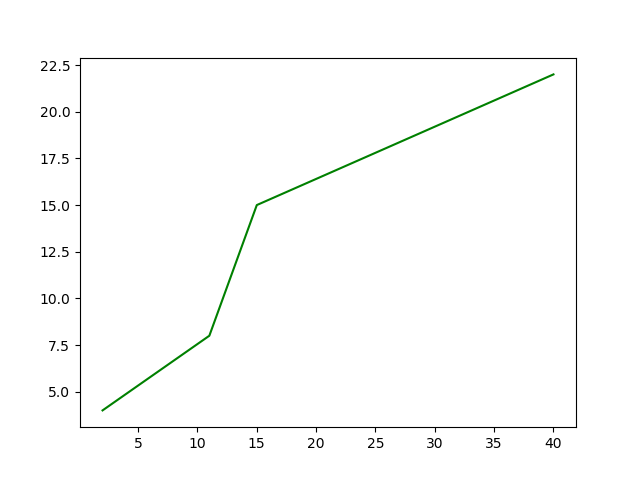
\includegraphics[keepaspectratio,alt={image.png}]{13c2e0a9-801f-4c40-9cf0-52b20d5ade04.png}}
\caption{image.png}
\end{figure}

The \texttt{plot()} function actually constructs the plot with its
elements. The \texttt{show()} function is what displays the plot to us
when we run the code.

Pyplot mimics aspects of MATLAB's plotting style, meaning that you can
style the plot with a series of style commands. One of the style
commands is color, which we saw above.

You can also change the symbols used to plot the variables. By default,
a solid line is drawn, but you can select other symbols like circles,
squares, or triangles.

You can pass the color and symbol instructions in as the third argument
of the call to construct the plot. You can view some of the various
options for plotting symbols here².

You can use \texttt{-\/-} to create dashes, s for squares, or
\texttt{\^{}} for triangles. For colors, you can use \texttt{r} for red,
\texttt{b} for blue, and \texttt{g} for green.

Here's how we could create a plot with green squares:

\begin{Shaded}
\begin{Highlighting}[]
    \DecValTok{1}\NormalTok{ plt.plot([}\DecValTok{2}\NormalTok{, }\DecValTok{11}\NormalTok{, }\DecValTok{15}\NormalTok{, }\DecValTok{40}\NormalTok{], [}\DecValTok{4}\NormalTok{, }\DecValTok{8}\NormalTok{, }\DecValTok{15}\NormalTok{, }\DecValTok{22}\NormalTok{], }\StringTok{\textquotesingle{}gs\textquotesingle{}}\NormalTok{)}
    \DecValTok{2}\NormalTok{ plt.show()}
\end{Highlighting}
\end{Shaded}

\begin{figure}
\centering
\pandocbounded{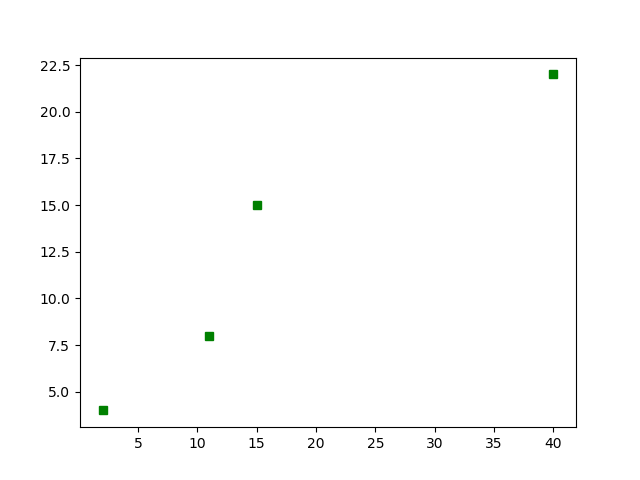
\includegraphics[keepaspectratio,alt={image.png}]{f7bdac4d-1a7c-4f0d-81d1-8bb39eaaa298.png}}
\caption{image.png}
\end{figure}

The plots we made above were continuous variables, now we'll explore how
to create plots using categorical variables.

You can plot categorical variables by specifying the different
categories and values in the form of lists and then passing those
variables to the adequate plotting function. For example, bar charts are
commonly used for categorical values.

Let's create and plot a bar chart:

\begin{Shaded}
\begin{Highlighting}[]
    \DecValTok{1}\NormalTok{ names }\OperatorTok{=}\NormalTok{ [}\StringTok{\textquotesingle{}A\textquotesingle{}}\NormalTok{, }\StringTok{\textquotesingle{}B\textquotesingle{}}\NormalTok{, }\StringTok{\textquotesingle{}C\textquotesingle{}}\NormalTok{]}
    \DecValTok{2}\NormalTok{ values }\OperatorTok{=}\NormalTok{ [}\DecValTok{19}\NormalTok{, }\DecValTok{50}\NormalTok{, }\DecValTok{29}\NormalTok{]}
    \DecValTok{3}
    \DecValTok{4}\NormalTok{ plt.bar(names, values)}
    \DecValTok{5}\NormalTok{ plt.show()}
\end{Highlighting}
\end{Shaded}

\begin{figure}
\centering
\pandocbounded{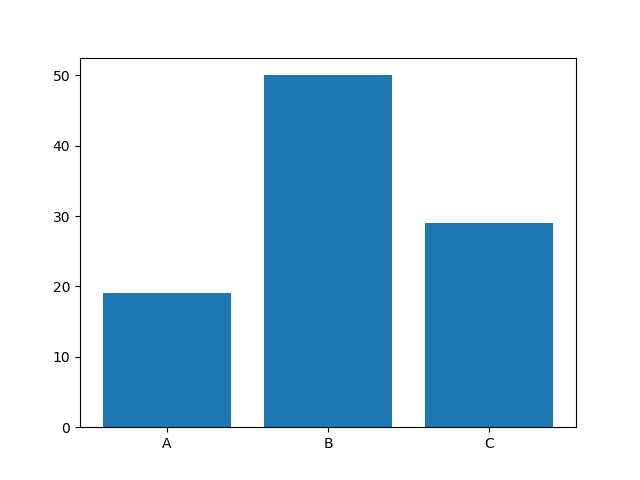
\includegraphics[keepaspectratio,alt={image.png}]{0d9f38ec-d5bd-4b98-a80d-f03e5918779c.png}}
\caption{image.png}
\end{figure}

There's an alternate way of creating plots with Matplotlib. The method
above allows you to quickly create plots, but if you want more control
over how the plot is created, you can create a \texttt{Figure} object
yourself.

Without creating a \texttt{Figure} object, Matplotlib creates a default
one for you, with the default settings. To change them, you can use the
\texttt{figure()} function of the \texttt{pyplot} module to create a
figure and then specify some properties. For example, you can set the
dimensions of the figure you want to create. The dimensions are passed
in using a list with four values between \texttt{0} and \texttt{1}.

The four numbers specify the dimensions in this order: left, bottom,
width, height. You can also do this with the \texttt{add\_subplot()}
function, discussed below.

Let's create a figure and add some information regarding the axes.

\subsubsection{Axes}\label{axes}

\texttt{Axes} objects sit within the figure you have created. Creating
an axes object will give you greater control over how data is visualized
and other elements of the plot are created.

When using an axes object, you can control how individual subplots are
displayed on those axes. You can think of it like this: Figures hold
axes and every axes object can store its own plots. The \texttt{Axes}
instance will contain most of the elements of a figure and you can have
multiple \texttt{Axes} for a single figure.

These elements include ticks, lines, text, polygons, etc. We'll explore
how to change these elements throughout the Customizing a Plot section,
up ahead. For now, let's just create an axes object on a figure:

\begin{Shaded}
\begin{Highlighting}[]
    \DecValTok{1}\NormalTok{ fig }\OperatorTok{=}\NormalTok{ plt.figure()}
    \DecValTok{2}\NormalTok{ ax }\OperatorTok{=}\NormalTok{ fig.add\_axes([}\DecValTok{0}\NormalTok{, }\DecValTok{0}\NormalTok{, }\DecValTok{1}\NormalTok{, }\DecValTok{1}\NormalTok{])}
    \DecValTok{3}\NormalTok{ names }\OperatorTok{=}\NormalTok{ [}\StringTok{\textquotesingle{}A\textquotesingle{}}\NormalTok{, }\StringTok{\textquotesingle{}B\textquotesingle{}}\NormalTok{, }\StringTok{\textquotesingle{}C\textquotesingle{}}\NormalTok{]}
    \DecValTok{4}\NormalTok{ values }\OperatorTok{=}\NormalTok{ [}\DecValTok{19}\NormalTok{, }\DecValTok{50}\NormalTok{, }\DecValTok{29}\NormalTok{]}
    \DecValTok{5}\NormalTok{ ax.bar(names, values)}
    \DecValTok{6}\NormalTok{ plt.show()}
\end{Highlighting}
\end{Shaded}

\begin{figure}
\centering
\pandocbounded{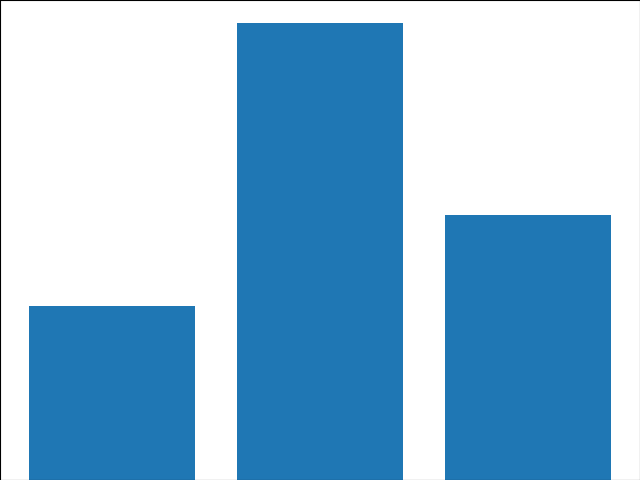
\includegraphics[keepaspectratio,alt={image.png}]{3b70e3bd-c6e1-4a5c-9570-776fb2292f3d.png}}
\caption{image.png}
\end{figure}

The \texttt{fig.add\_axes()} function returns a new \texttt{Axes} object
which we've packed in ax. Using this object, we'll be adding elements.
For example, we've called \texttt{ax.bar()} to plot a bar graph instead
of calling \texttt{plt.bar()} like before.

\texttt{ax} belongs to the \texttt{fig} so everything added to the
\texttt{ax} will also be added to the \texttt{fig}. The arguments we've
passed to the \texttt{add\_axes()} function were
\texttt{{[}0,\ 0,\ 1,\ 1{]}}. These are the \texttt{left},
\texttt{bottom}, \texttt{width}, and \texttt{height} of the \texttt{ax}
object.

The numbers are fractions of the figure the \texttt{Axes} object belongs
to, so we've told it to start at the bottom-left point (\texttt{0} for
\texttt{left} and \texttt{0} for \texttt{bottom}) and to have the same
height and width of the parent figure (\texttt{1} for \texttt{width} and
\texttt{1} for \texttt{height}).

We can't really see the \texttt{ax} at this point, other than the plot
is missing some elements as opposed to the previous example where they
were set to default.

You can also delete axes through the use of the \texttt{delaxes()}
function:

\begin{Shaded}
\begin{Highlighting}[]
    \DecValTok{1}\NormalTok{ fig.delaxes(ax)}
\end{Highlighting}
\end{Shaded}

Now that we know the general method for creating plots in Matplotlib,
let's take a look at the many options you have at your disposal for
customizing these plots.

\subsubsection{Subplots}\label{subplots}

Matplotlib allows you to create multiple plots within the same figure.
In order to add multiple plots, you need to create a ``subplot'' for
each plot in the figure you'd like to use.

This is done with the \texttt{add\_subplot()} function, which accepts a
series of numeric arguments.

The first number specifies how many rows you want to add to the figure,
the second number specifies how many columns you want to add, and the
third number specifies the number of the plot that you want to add.

This means that if you in passed in \texttt{111} into the
\texttt{add\_subplots()} function, one new subplot would be added to the
figure. Meanwhile, if you used the numbers \texttt{221}, the resulting
plot would have four axes with two columns and two rows - and the
subplot you're forming is in the 1st position.

Here's how we would create two subplots in the same figure, notice that
we have created two axes objects:

\begin{Shaded}
\begin{Highlighting}[]
    \DecValTok{1}\NormalTok{ fig }\OperatorTok{=}\NormalTok{ plt.figure()}
    \DecValTok{2}
    \DecValTok{3}\NormalTok{ names }\OperatorTok{=}\NormalTok{ [}\StringTok{\textquotesingle{}A\textquotesingle{}}\NormalTok{, }\StringTok{\textquotesingle{}B\textquotesingle{}}\NormalTok{, }\StringTok{\textquotesingle{}C\textquotesingle{}}\NormalTok{]}
    \DecValTok{4}\NormalTok{ values }\OperatorTok{=}\NormalTok{ [}\DecValTok{19}\NormalTok{, }\DecValTok{50}\NormalTok{, }\DecValTok{29}\NormalTok{]}
    \DecValTok{5}\NormalTok{ values\_2 }\OperatorTok{=}\NormalTok{ [}\DecValTok{48}\NormalTok{, }\DecValTok{19}\NormalTok{, }\DecValTok{41}\NormalTok{]}
    \DecValTok{6}
    \DecValTok{7}\NormalTok{ ax }\OperatorTok{=}\NormalTok{ fig.add\_subplot(}\DecValTok{121}\NormalTok{)}
    \DecValTok{8}\NormalTok{ ax2 }\OperatorTok{=}\NormalTok{ fig.add\_subplot(}\DecValTok{122}\NormalTok{)}
    \DecValTok{9}
    \DecValTok{10}\NormalTok{ ax.bar(names, values)}
    \DecValTok{11}\NormalTok{ ax2.bar(names, values\_2)}
    \DecValTok{12}\NormalTok{ plt.show()}
\end{Highlighting}
\end{Shaded}

\begin{figure}
\centering
\pandocbounded{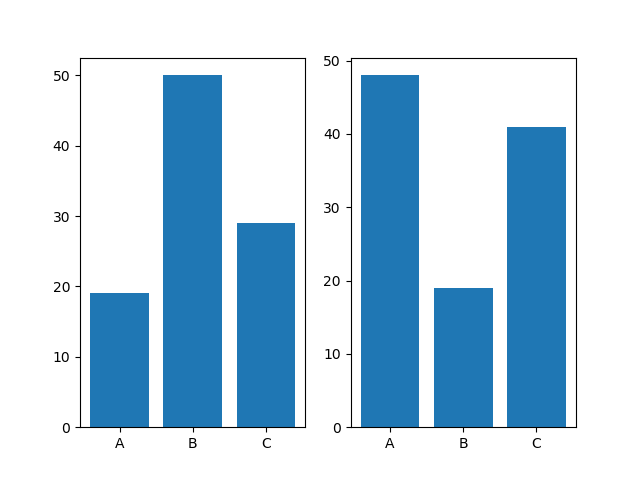
\includegraphics[keepaspectratio,alt={image.png}]{3e59d7b4-1e36-4d33-a51f-60f53da78999.png}}
\caption{image.png}
\end{figure}

We've created two sublots in a figure with 1 row and 2 columns. They're
sitting side by side. If we had created a figure with 2 rows and 1
column:

\begin{Shaded}
\begin{Highlighting}[]
    \DecValTok{1}\NormalTok{ fig }\OperatorTok{=}\NormalTok{ plt.figure()}
    \DecValTok{2}
    \DecValTok{3}\NormalTok{ names }\OperatorTok{=}\NormalTok{ [}\StringTok{\textquotesingle{}A\textquotesingle{}}\NormalTok{, }\StringTok{\textquotesingle{}B\textquotesingle{}}\NormalTok{, }\StringTok{\textquotesingle{}C\textquotesingle{}}\NormalTok{]}
    \DecValTok{4}\NormalTok{ values }\OperatorTok{=}\NormalTok{ [}\DecValTok{19}\NormalTok{, }\DecValTok{50}\NormalTok{, }\DecValTok{29}\NormalTok{]}
    \DecValTok{5}\NormalTok{ values\_2 }\OperatorTok{=}\NormalTok{ [}\DecValTok{48}\NormalTok{, }\DecValTok{19}\NormalTok{, }\DecValTok{41}\NormalTok{]}
    \DecValTok{6}
    \DecValTok{7}\NormalTok{ ax }\OperatorTok{=}\NormalTok{ fig.add\_subplot(}\DecValTok{211}\NormalTok{)}
    \DecValTok{8}\NormalTok{ ax2 }\OperatorTok{=}\NormalTok{ fig.add\_subplot(}\DecValTok{212}\NormalTok{)}
    \DecValTok{9}
    \DecValTok{10}\NormalTok{ ax.bar(names, values)}
    \DecValTok{11}\NormalTok{ ax2.bar(names, values\_2)}
    \DecValTok{12}\NormalTok{ plt.show()}
\end{Highlighting}
\end{Shaded}

We'd be looking at something like this:

\begin{figure}
\centering
\pandocbounded{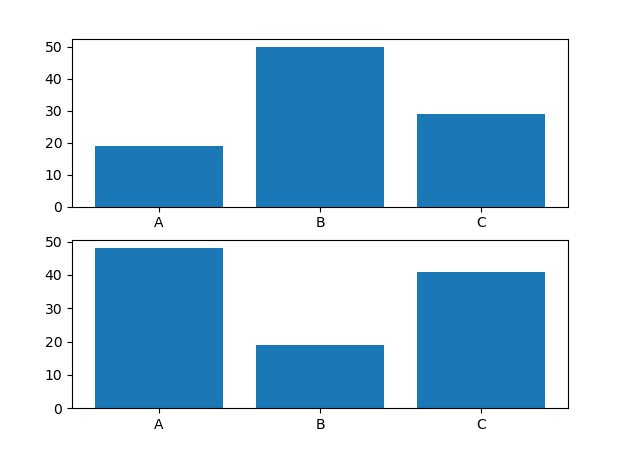
\includegraphics[keepaspectratio,alt={image.png}]{75ee4540-68fc-46ed-9c0b-d2938fe31d40.png}}
\caption{image.png}
\end{figure}


    % Add a bibliography block to the postdoc
    
    
    
\end{document}
